\documentclass[final,hyperref={pdfpagelabels=false},xcolor=dvipsnames]{beamer}
\mode<presentation>
  {
  %  \usetheme{Berlin}
  \usetheme{FUBerlin}
  \usecolortheme{orchid}
%\usetheme{TUGraz}
  }
  \usepackage{times}
  \usepackage{amsmath,amsthm, amssymb, latexsym, fancyvrb}
  \boldmath
  \usepackage[english]{babel}
  \usepackage[latin1]{inputenc}
  \usepackage[orientation=portrait,size=a0,scale=1.4,debug]{beamerposter}


  \usepackage{stmaryrd}
  \newcommand{\typearrow}{\shortrightarrow}
  \newcommand{\itype}{\iota}
  \newcommand{\utype}{u}
  \newcommand{\proptype}{\tau}
  \newcommand{\exInW}{eiw}
  \newcommand{\chriscite}[1]{\textcolor{darkgray}{\textit{\scriptsize Reading:
        #1}}}
  \newcommand{\qcl}{QCL}

  \newcommand{\holpp}{\textcolor{brown}{H}}
  \newcommand{\holp}{\textcolor{brown}{$\holpp$}}
  \newcommand{\holpLeo}{\textcolor{brown}{$\holpp_{L}$}}
  \newcommand{\holpSatallax}{\textcolor{brown}{$\holpp_{S}$}}
  \newcommand{\holpIsabelle}{\textcolor{brown}{$\holpp_{I}$}}
  \newcommand{\holpNitpick}{\textcolor{brown}{$\holpp_{N}$}}
  \newcommand{\holpAgsyhol}{\textcolor{brown}{$\holpp_{A}$}}
  \newcommand{\holpLSA}{\textcolor{brown}{$\holpp_{A,L,S}$}}
  \newcommand{\holpLS}{\textcolor{brown}{$\holpp_{L,S}$}}
  \newcommand{\holpLA}{\textcolor{brown}{$\holpp_{A,L}$}}
  \newcommand{\holpSA}{\textcolor{brown}{$\holpp_{A,S}$}}

  %%%%%%%%%%%%%%%%%%%%%%%%%%%%%%%%%%%%%%%%%%%%%%%%%%%%%%%%%%%%%%%%%%%%%%%%%%%%%%%%%5
  \graphicspath{{figures/}}
  \title[Automating Quantified Conditional Logics in HOL]{The
    Inconsistency in \\ G{\"o}del's Ontological Argument \\
--- A Success Story for AI in Metaphysics ---}
  \author[]{Christoph Benzm{\"u}ller$^1$ and Bruno Woltzenlogel Paleo}
  \institute[]{{\footnotesize $^1$Supported by the German Research Foundation   (grant BE2501/12-1,2)}}
  %\date{Jul. 31th, 2007}


  %%%%%%%%%%%%%%%%%%%%%%%%%%%%%%%%%%%%%%%%%%%%%%%%%%%%%%%%%%%%%%%%%%%%%%%%%%%%%%%%%5
  \begin{document}
  \begin{frame}{}
  \vskip-3ex
    \begin{columns}[t]
      \begin{column}{.49\linewidth}
        \begin{block}{\large Motivation} 
          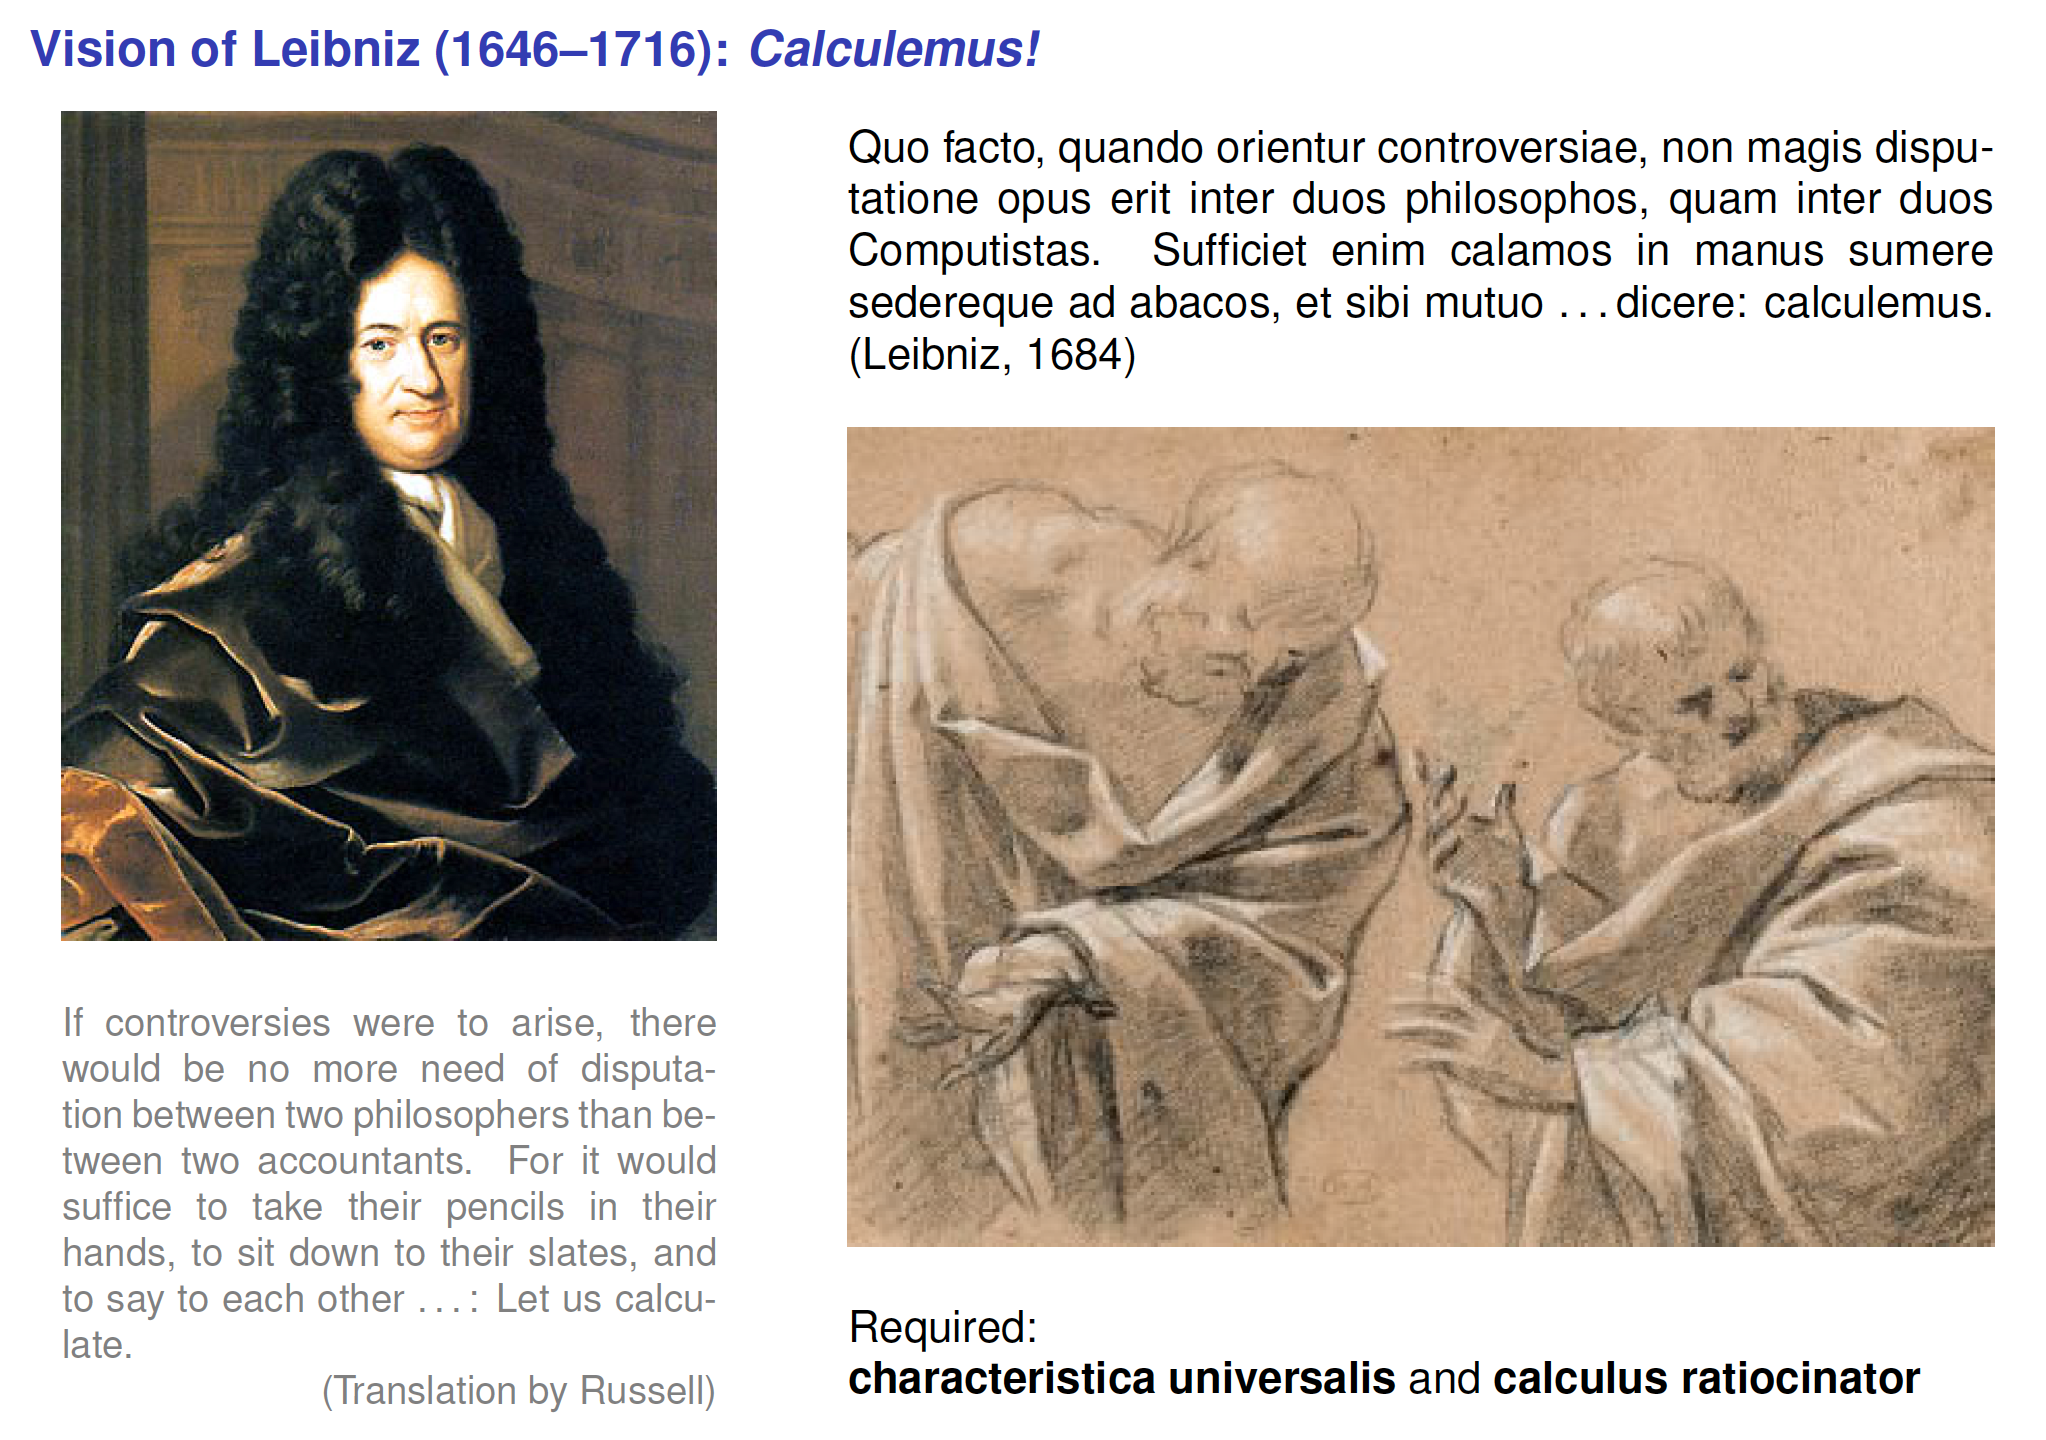
\includegraphics[width=0.98\textwidth]{./Images/VisionLeibniz}
        \end{block}
      \end{column}
      \hfill
      \begin{column}{.48\linewidth}
        \begin{block}{\large Application: G�del's Ontological
            Argument} \centering
           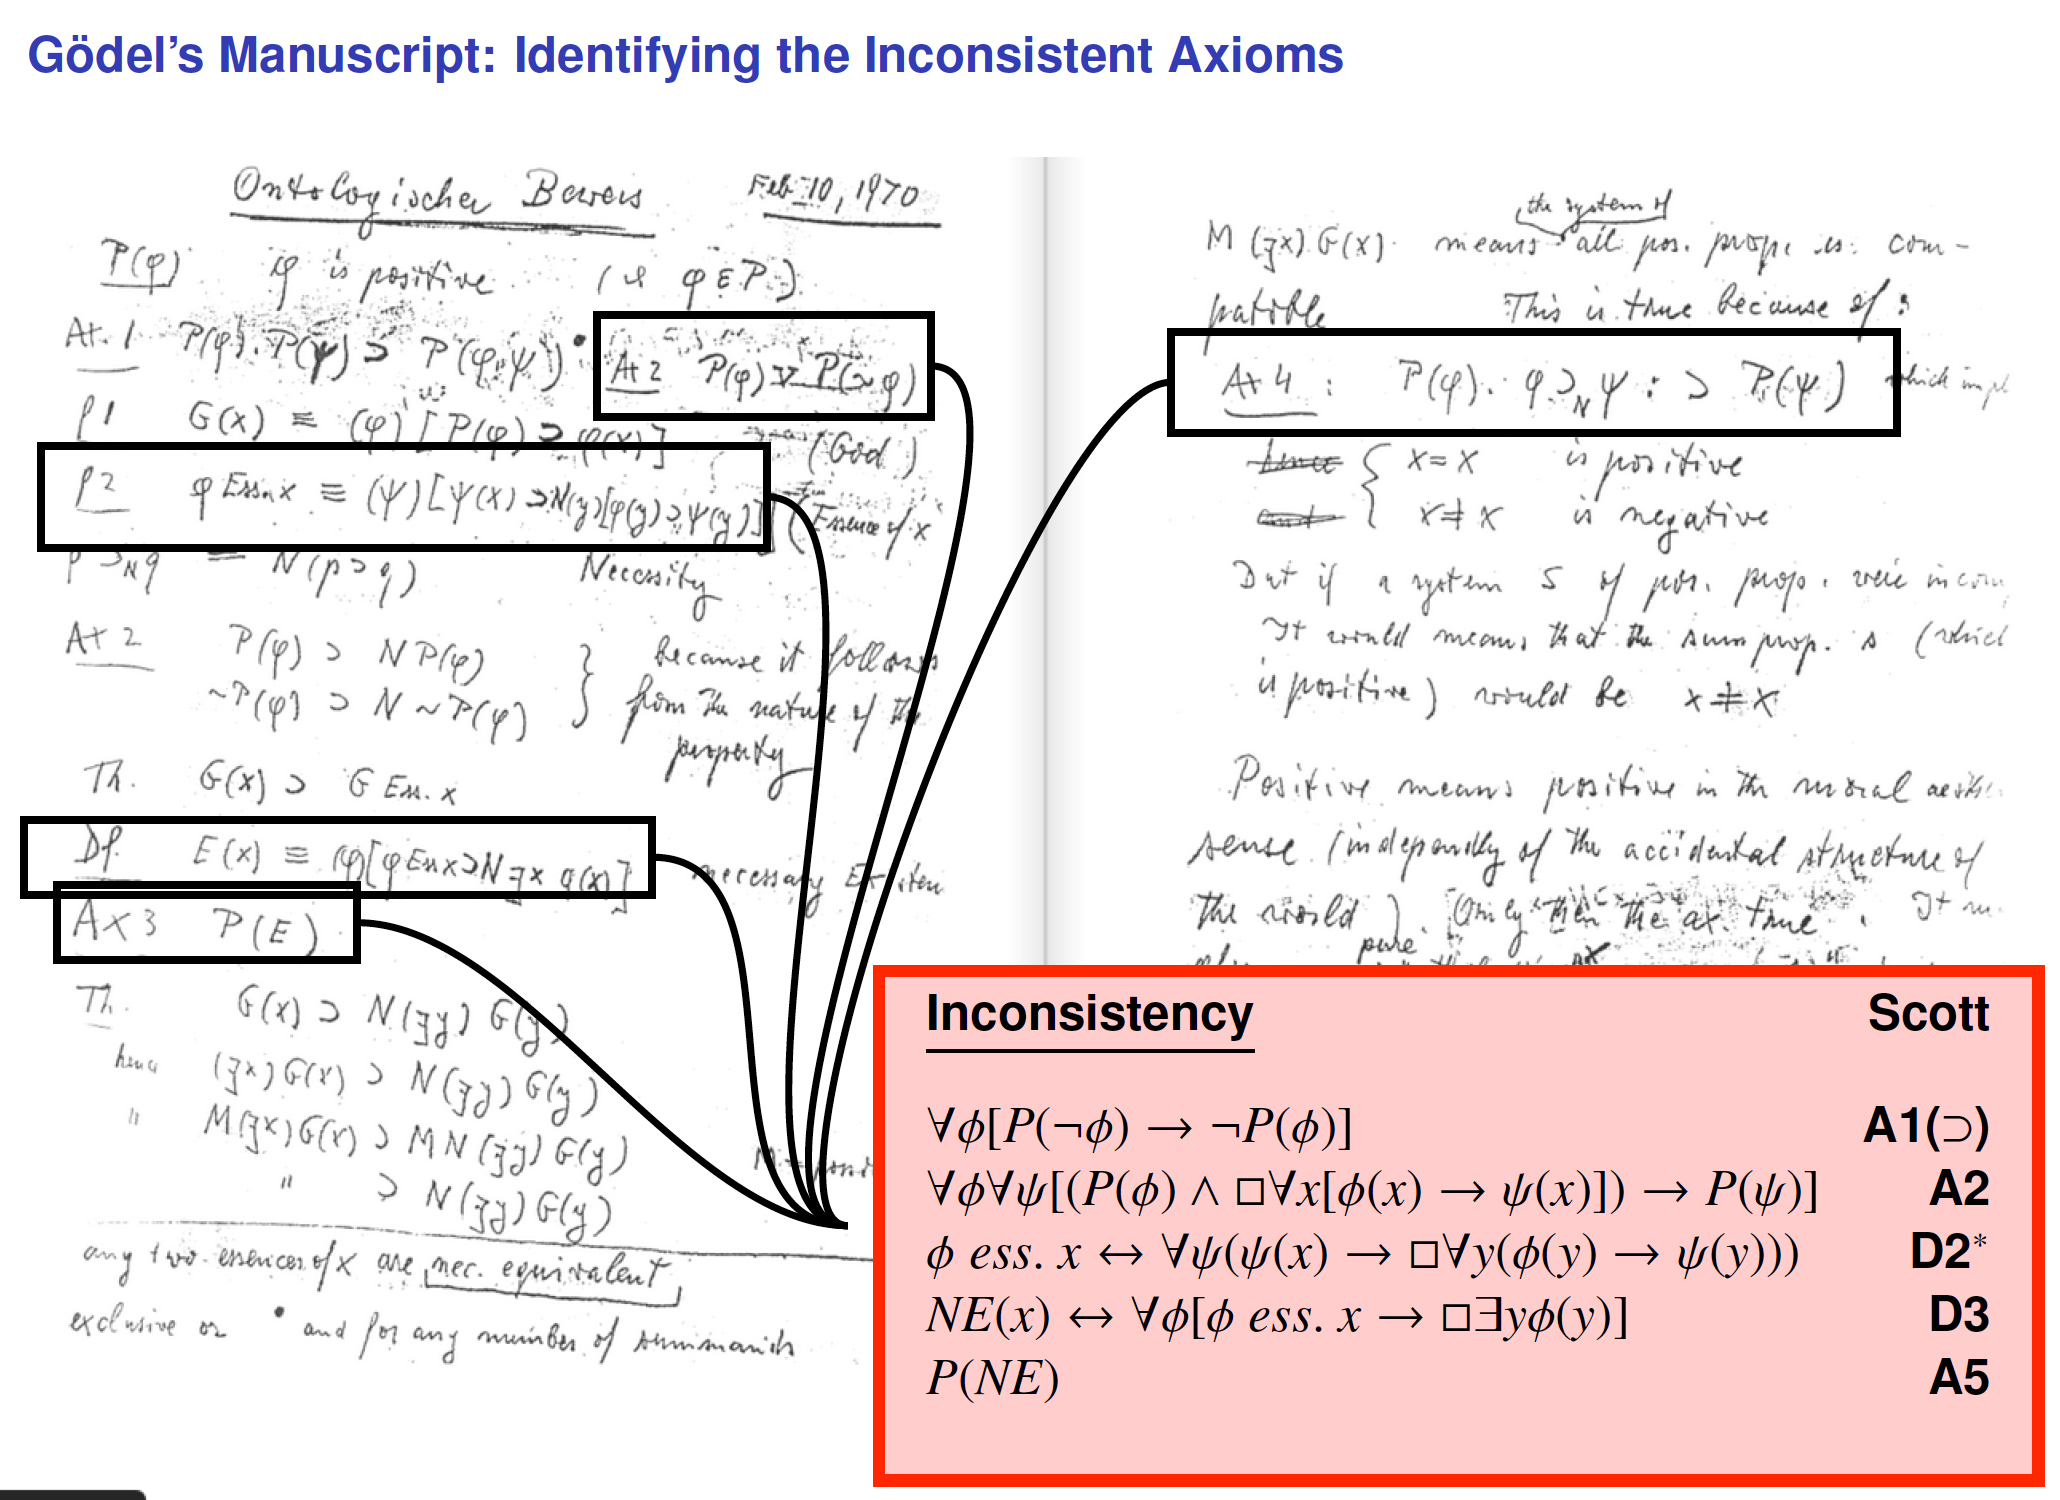
\includegraphics[width=0.98\textwidth]{./Images/GoedelInconsistency}
        \end{block}
      \end{column}
    \end{columns} \vskip-3ex
    \begin{columns}[t]
      \begin{column}{.33\linewidth}
        \begin{block}{\large Difference between Scott's and G�del's Versions} 
          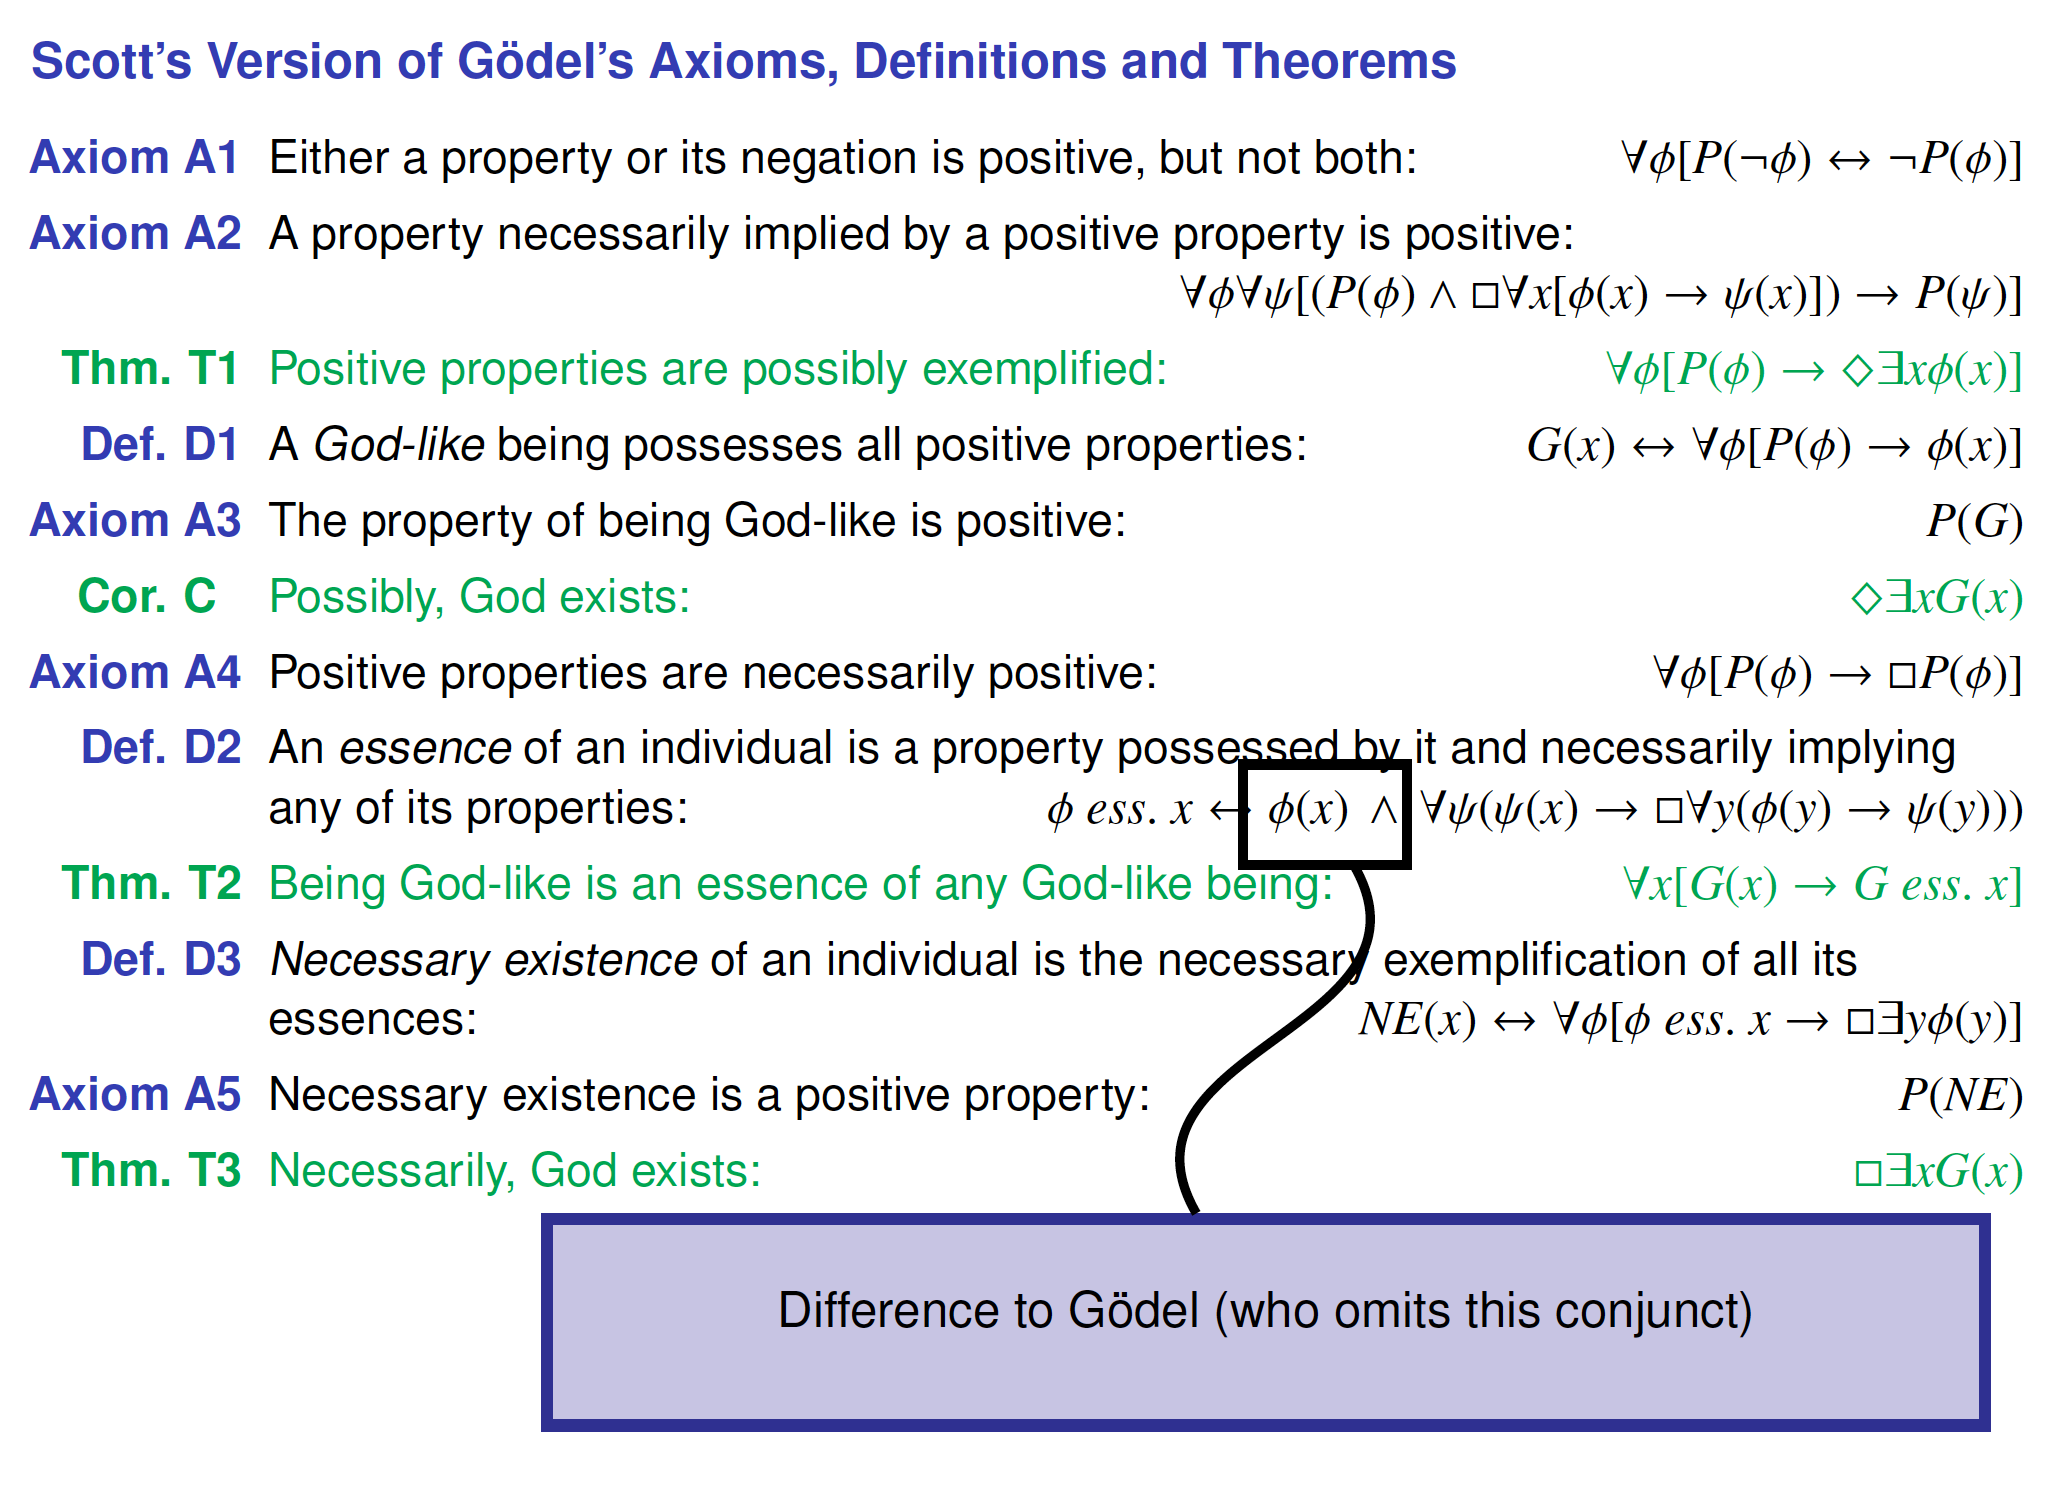
\includegraphics[width=0.98\textwidth]{./Images/Scott_vs_Goedel}
        \end{block}
      \end{column}
      \hfill
      \begin{column}{.33\linewidth}
        \begin{block}{\large Approach: Semantic Embedding}
          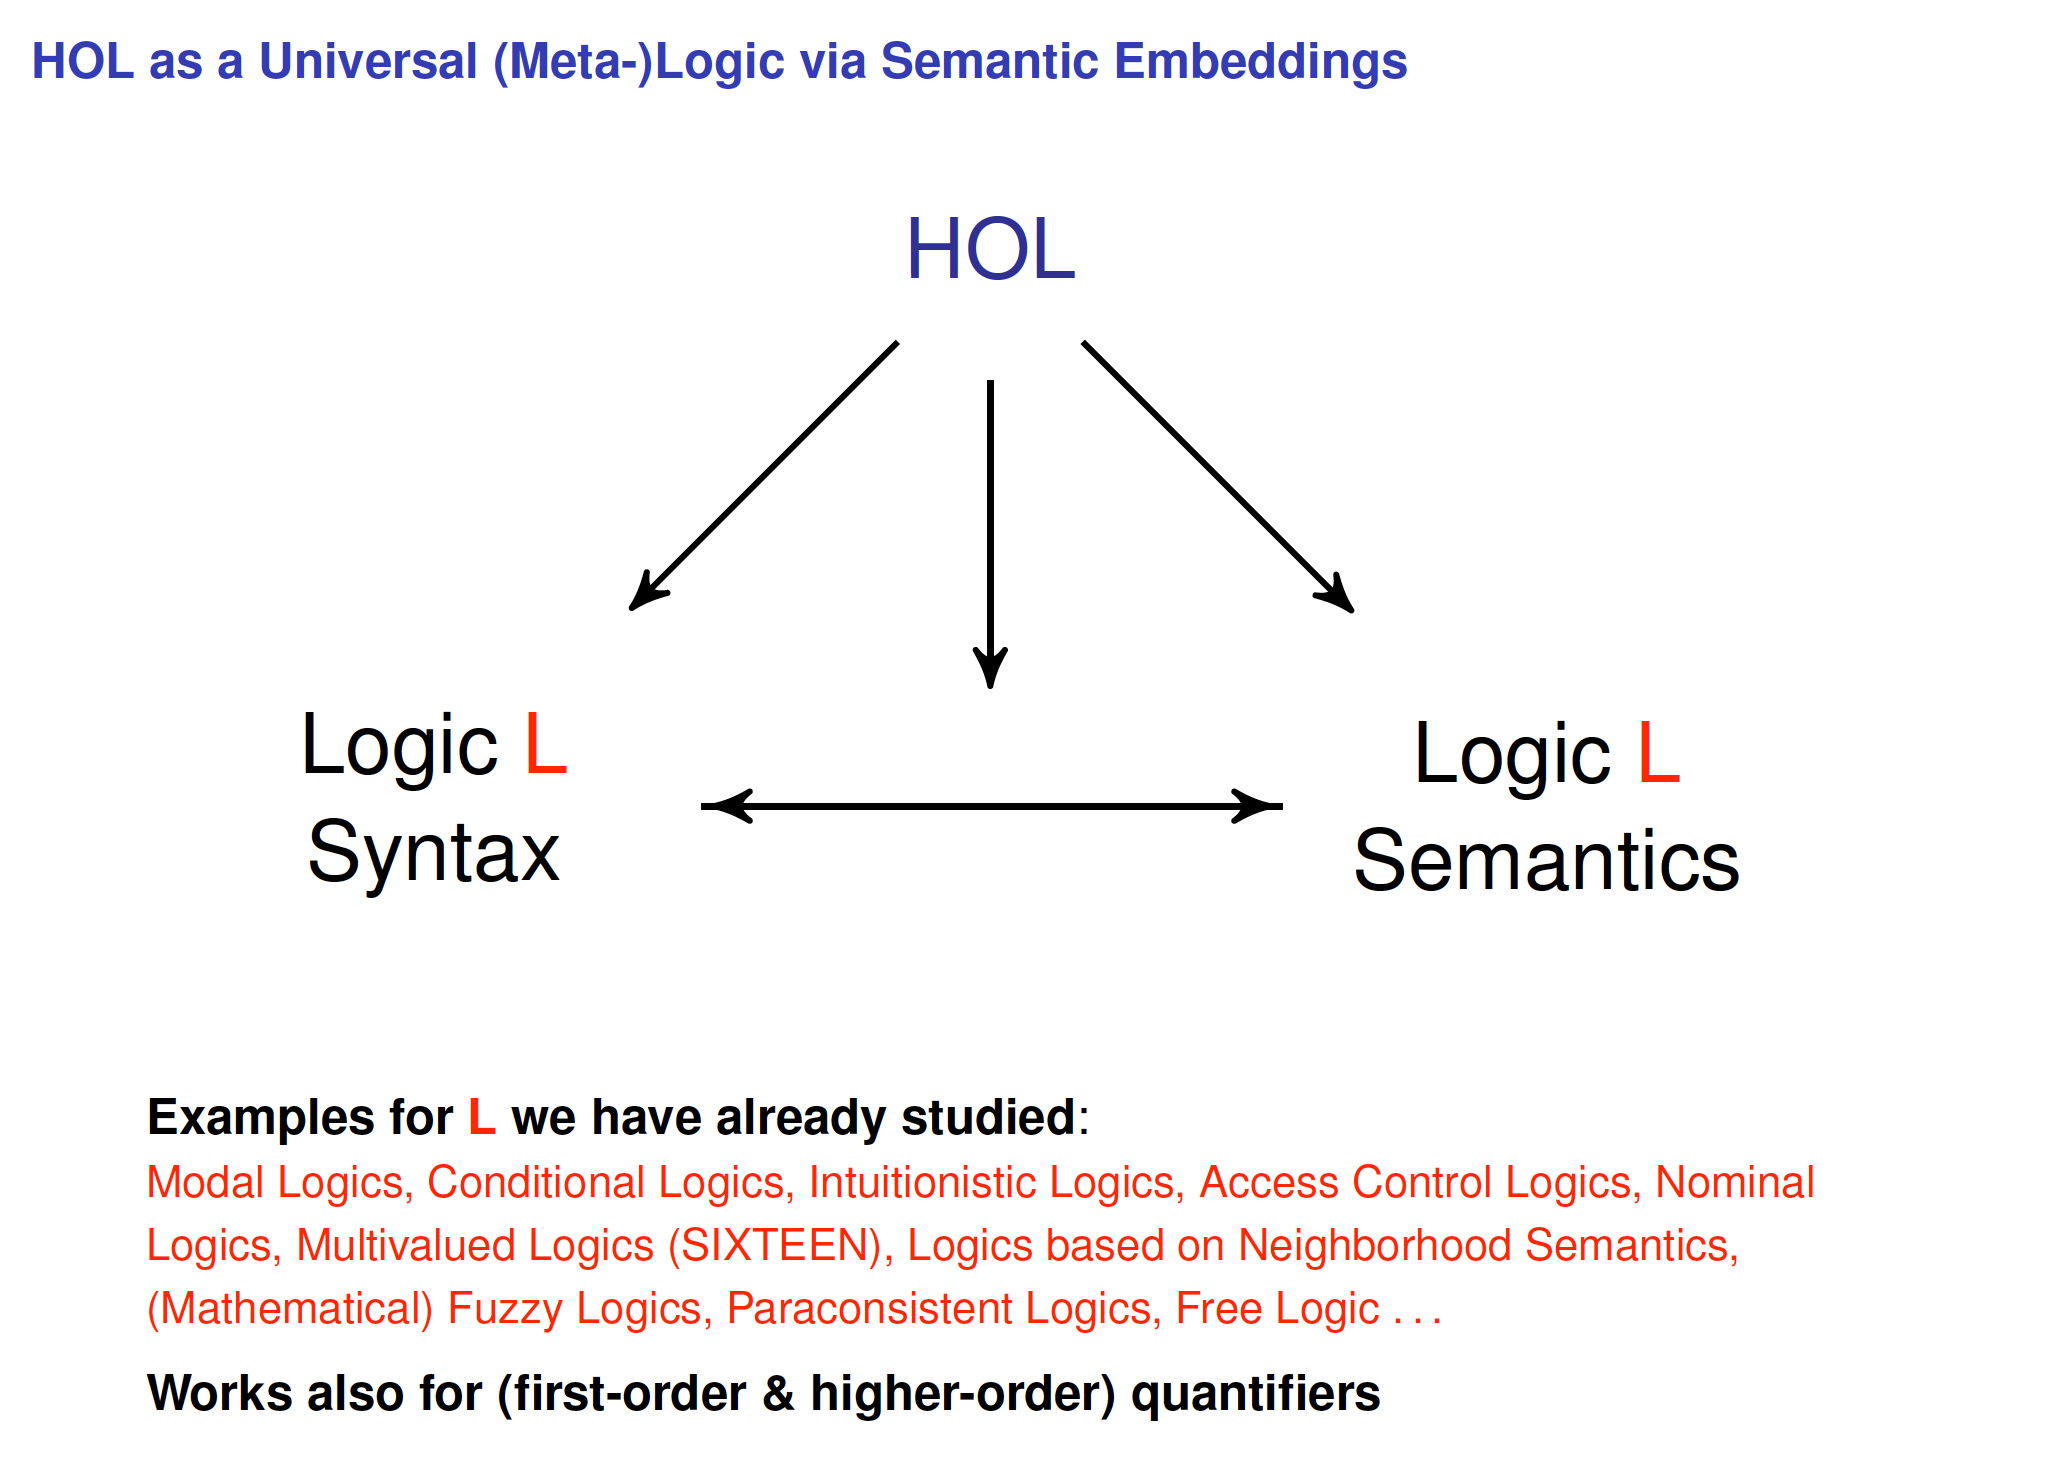
\includegraphics[width=0.98\textwidth]{./Images/SemanticEmbedding}
        \end{block}
      \end{column}
     \begin{column}{.33\linewidth}
        \begin{block}{\large Bla}
           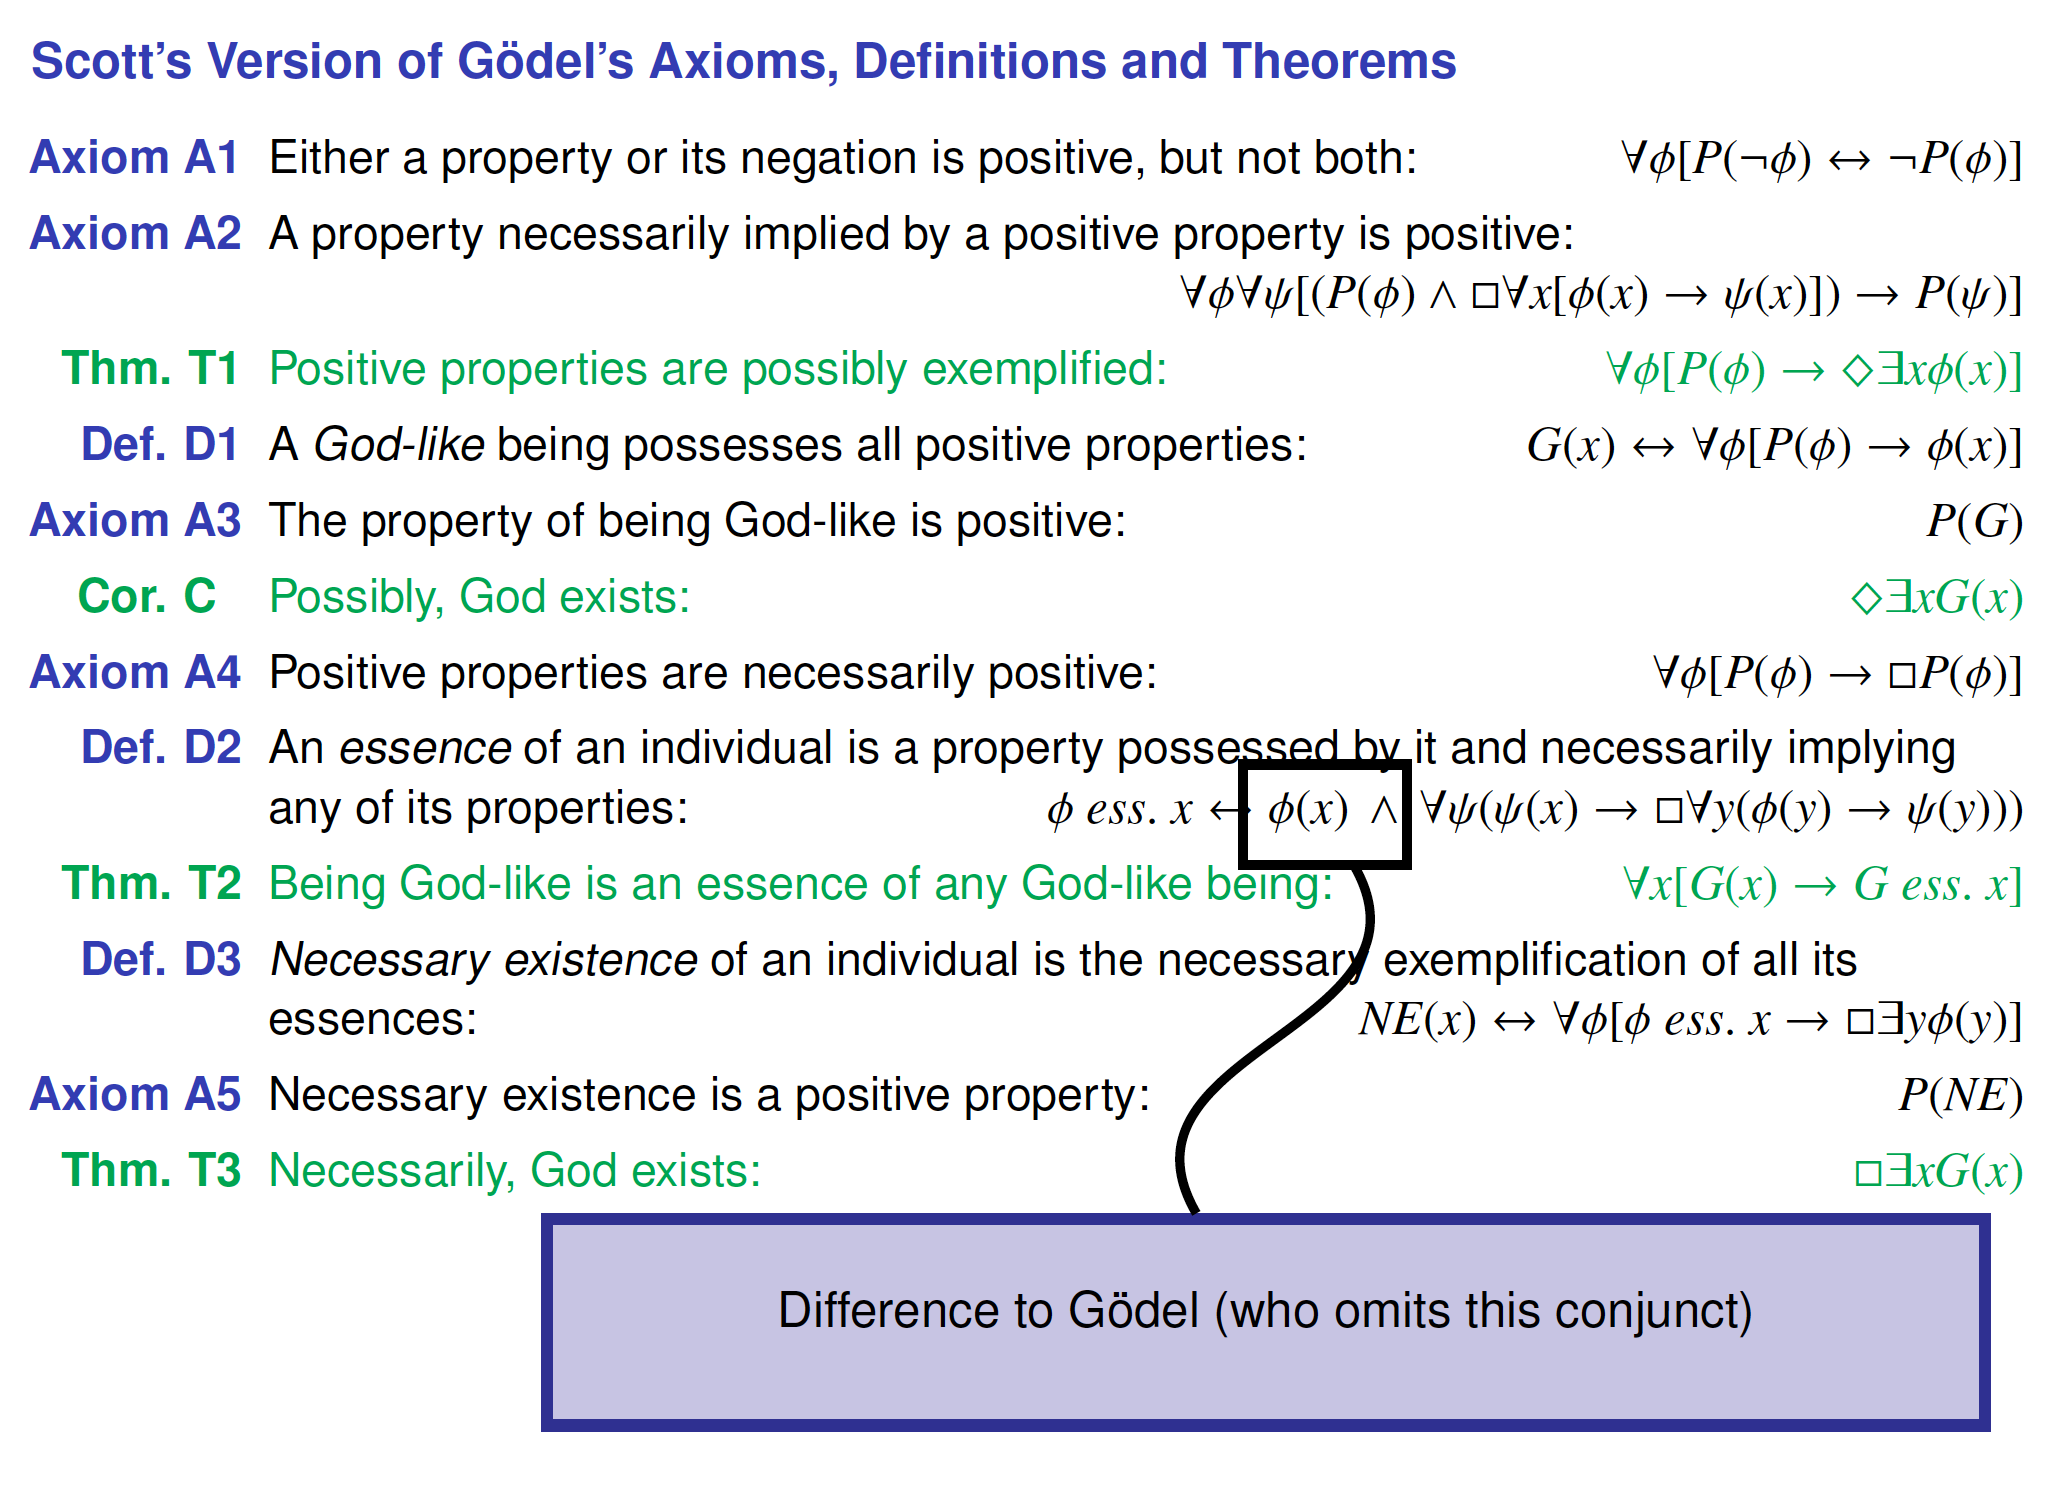
\includegraphics[width=0.98\textwidth]{./Images/Scott_vs_Goedel}
        \end{block}
      \end{column}
    \end{columns} \vskip-3ex
 \end{frame}
\end{document}


%%%%%%%%%%%%%%%%%%%%%%%%%%%%%%%%%%%%%%%%%%%%%%%%%%%%%%%%%%%%%%%%%%%%%%%%%%%%%%%%%%%%%%%%%%%%%%%%%%%%
%%% Local Variables: 
%%% mode: latex
%%% TeX-PDF-mode: t
%%% End:
